\chapter{Feedback}

\section{Basic Feedback Structure}

\begin{figure}[H]
  \centering
  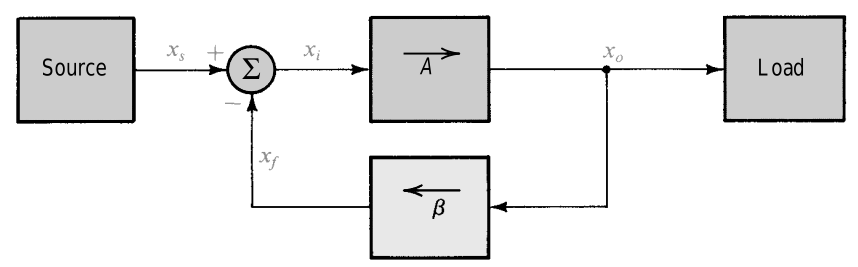
\includegraphics[width=0.9\linewidth]{figures/Basic-Feedback-Structure}
\end{figure}

\begin{equation*}
  \begin{aligned}
    x_o = A x_i \quad\quad x_f = \beta x_o \quad\quad x_i = x_s - x_f
  \end{aligned}
\end{equation*}

\begin{equation*}
  \begin{aligned}
    A_f = \dfrac{x_0}{x_s}  = \dfrac{A x_i}{x_i + \beta A x_i } = \dfrac{A}{1 + A \beta} \approx \dfrac{1}{\beta}  \quad\quad \left( A\beta \gg 1 \right)
  \end{aligned}
\end{equation*}

\section{Bandwidth and Gain}

\begin{figure}[H]
  \centering
  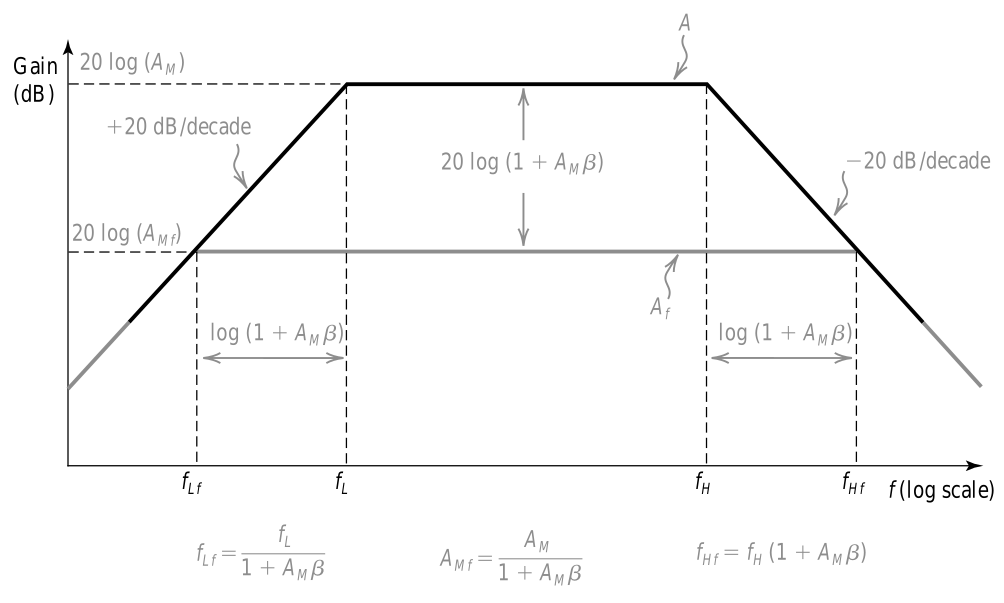
\includegraphics[width=0.6\linewidth]{figures/Feedback-Bandwidth}
  \label{fig:}
\end{figure}

\begin{equation*}
  \begin{aligned}
    \omega_{Hf} = \omega_H \cdot \left( 1 + A_M \beta \right) \quad\quad \omega_{Lf} = \omega_L / \left( 1 + A_M \beta \right)
  \end{aligned}
\end{equation*}

\section{Stability Problem of Feedback}

\begin{figure}[H]
  \centering
  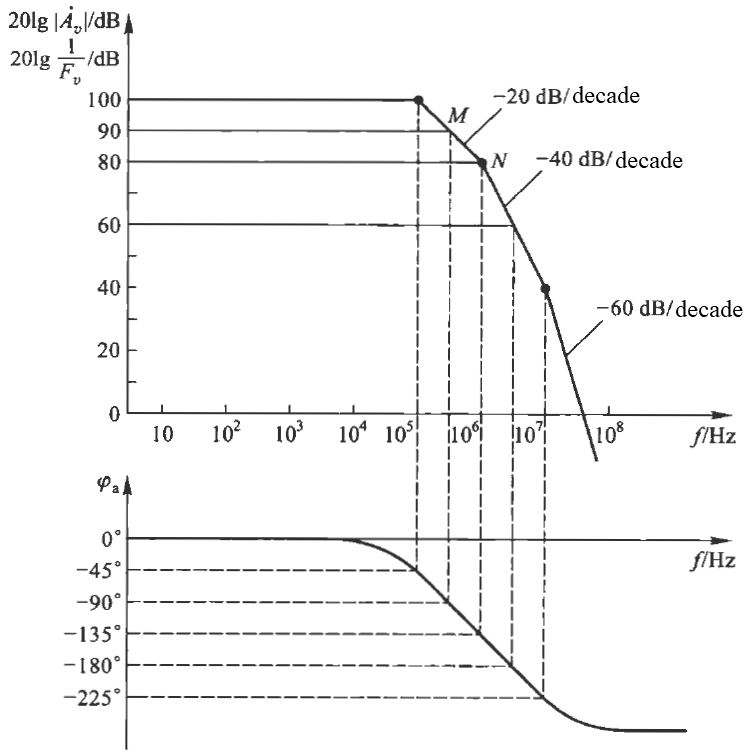
\includegraphics[width=0.8\linewidth]{figures/Stability-Feedback}
\end{figure}

\begin{equation*}
  \begin{aligned}
    \varphi_{a} = -135^{\circ} \quad\quad AF < 1
  \end{aligned}
\end{equation*}

\section{Four Basic Feedback Topologies}

\begin{table*}[h]
  \centering
  \begin{tabular}{|Sc|Sc|Sc|Sc|Sc|}
    \hline
    Feedback Type & Usage & Gain & Input Resistance & Output Resistance \\
    \hline
    Series-Shunt & Voltage $\rightarrow$ Voltage & $A_f = \dfrac{A}{1 + A \beta} $ & $ R_{if} = \left( 1 + A \beta \right) R_i$ & $R_{of} = \dfrac{R_o}{1 + A \beta} $ \\
    \hline
    Shunt-Series & Current $\rightarrow$ Current & $A_f = \dfrac{A}{1 + A \beta} $ & $ R_{if} = \dfrac{R_i}{1 + A \beta} $ & $R_{of} = \left( 1 + A \beta \right) R_o $ \\
    \hline
    Series-Series & Voltage $\rightarrow$ Current & $A_f = \dfrac{A}{1 + A \beta} $ & $ R_{if} = \left( 1 + A \beta \right) R_i$ & $R_{of} = \left( 1 + A \beta \right) R_o $ \\
    \hline
    Shunt-Shunt & Current $\rightarrow$ Voltage & $A_f = \dfrac{A}{1 + A \beta} $ & $ R_{if} = \dfrac{R_i}{1 + A \beta}  R_i$ & $R_{of} = \dfrac{R_o}{1 + A \beta} $ \\
    \hline
  \end{tabular}
\end{table*}

\section{Positive or Negative}

\begin{table*}[h]
  \centering
  \begin{tabular}{|Sc|Sc|Sc|Sc|Sc|Sc|Sc|}
    \hline
    Amplifier Type & Common S & Common G & Common D & Common E & Common B & Common C \\
    \hline
    Sign of $A_v$ & $-$ & $+$ & $+$ & $-$ & $+$ & $-$ \\
    \hline
  \end{tabular}
\end{table*}

\section{Virtual Short and Open Circuit of Amplifier in the State of Deep Negative Feedback}

\begin{figure}[H]
  \centering
  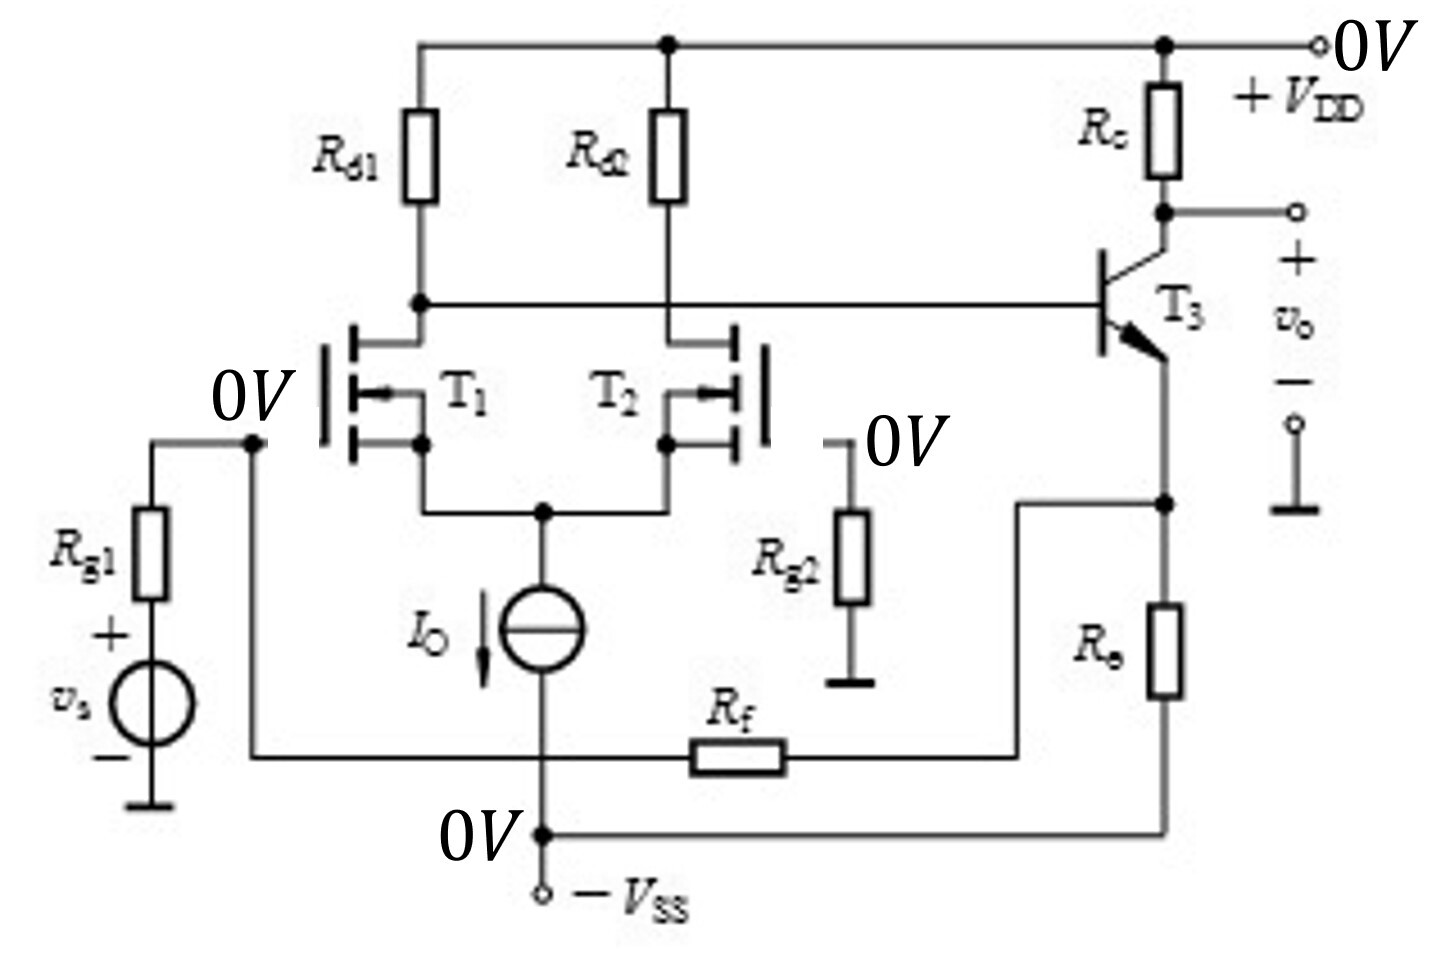
\includegraphics[width=0.9\linewidth]{figures/Feedback-Virtual-Short-Open-Circuit}
\end{figure}

%%% Local Variables:
%%% mode: latex
%%% TeX-master: "Analogue_Electronics"
%%% End:
